\begin{figure}[!ht]
    \centering
    a)
    \begin{minipage}{.45\textwidth}
        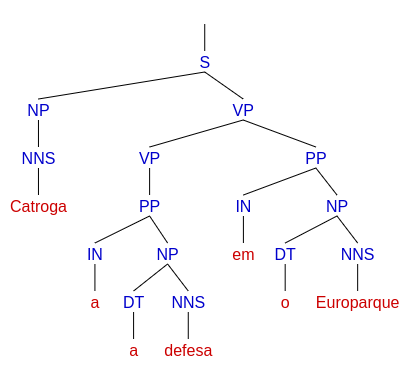
\includegraphics[width=\linewidth]{imagens/ec_cintil_sem_ponto_tree_trans.png}
    \end{minipage}
    % 
    b)
    \begin{minipage}{.45\textwidth}
        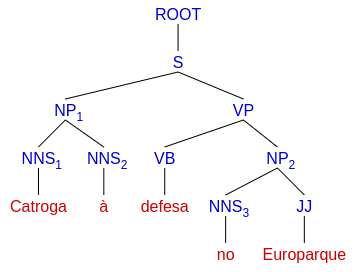
\includegraphics[width=\linewidth]{imagens/ec_cintil_sem_ponto_tree_sp.png}
    \end{minipage}
    \caption[Estudo de caso CINTIL - Sentença transduzida sem pontuação]{Estudo da sentença eCTMP-000647/78121, \textquote{Catroga à defesa no Europarque}, que originalmente não possui nenhuma pontuação. Em a), vemos a sentença no seu formato original no CINTIL. Em b), o resultado de sua transdução}
    \label{fig:ec_cintil_sem_ponto_tree}
\end{figure}